\documentclass[12pt,a4paper,catalan]{article}
\usepackage[utf8]{inputenc}
\usepackage[catalan]{babel}
\usepackage{amsmath}
\usepackage{amsfonts}
\usepackage{amssymb}
\usepackage{graphicx}
\usepackage{float}
\usepackage{framed}
\usepackage{url}
\usepackage{listings}
\usepackage{color}
\usepackage{textcomp}
\definecolor{lightgray}{rgb}{.9,.9,.9}
\definecolor{darkgray}{rgb}{.4,.4,.4}
\definecolor{purple}{rgb}{0.65, 0.12, 0.82}
\graphicspath{{images/}}
\lstdefinelanguage{JavaScript}{
	keywords={typeof, new, true, false, catch, function, return, null, catch, switch, var, const, let, if, in, while, do, else, case, break},
	keywordstyle=\color{blue}\bfseries,
	ndkeywords={class, static, extends, constructor, get, set, export, boolean, throw, implements, import, this},
	ndkeywordstyle=\color{darkgray}\bfseries,
	identifierstyle=\color{black},
	sensitive=false,
	comment=[l]{//},
	morecomment=[s]{/*}{*/},
	commentstyle=\color{purple}\ttfamily,
	stringstyle=\color{red}\ttfamily,
	morestring=[b]',
	morestring=[b]"
}
\lstset{
	language=JavaScript,
	backgroundcolor=\color{lightgray},
	extendedchars=true,
	basicstyle=\footnotesize\ttfamily,
	showstringspaces=false,
	showspaces=false,
	numbers=left,
	numberstyle=\footnotesize,
	numbersep=9pt,
	tabsize=2,
	breaklines=true,
	showtabs=false,
	captionpos=b
}
\usepackage[backend=biber,style=numeric,citestyle=numeric]{biblatex}
\addbibresource{bibliography.bib}
\author{Marc Ferrer Fontirroig}
\title{Rehabilitació complementària basada en videojocs utilitzant Leap Motion}
\begin{document}
	\thispagestyle{empty}
	\begin{center}
		
\includegraphics[scale=0.7]{uib-logo.jpg}
	\end{center}
	\begin{center}
		\textbf{ESCOLA POLITÈCNICA SUPERIOR}\\
		\textbf{UNIVERSITAT DE LES ILLES BALEARS}\\
		\vspace{3em}
		\textbf{\underline{\Large{PROJECTE FINAL DE CARRERA}}}\\
		\vspace{1.5em}
		\textbf{\large{Estudis:}}
		\begin{framed}
			\textbf{\large{ENGINYERIA INFORMÀTICA}}
		\end{framed}
		\textbf{\large{Títol}}
		\begin{framed}
			\textbf{REHABILITACIÓ COMPLEMENTÀRIA BASADA EN VIDEOJOCS UTILITZANT LEAP MOTION}
		\end{framed}
		\vspace{3em}
	\end{center}
	\begin{flushright}
		\textbf{Autor:} Marc Ferrer Fontirroig\\
		\textbf{Directora:} Cristina S. Manresa Yee\\
	\end{flushright}
	\textbf{Data:} 9 de juny de 2017
	\newpage
	\tableofcontents
	\newpage
	\listoffigures
	\newpage
	\noindent Cristina S. Manresa Yee, faig constar que he dirigit el Projecte de Final de Carrera titulat “Rehabilitació complementària basada en videojocs utilitzant Leap Motion” realitzat per l'alumne Marc Ferrer Fontirroig i que el treball està acabat i preparat per a la seva presentació pública.\\\\
	Palma,  dia de mes i any
	
	\vspace{3cm}
	
	\noindent Signat: Cristina S. Manresa Yee
	\newpage
	\section*{Resum}
	El projecte que es presenta descriu el desenvolupament d'una prova de concepte per a la utilització d'interfícies basades en visió per a la realització d'exercicis de rehabilitació física, que pugui servir com a teràpia complementària a la teràpia convencional amb un professional com pugui ser un fisioterapeuta.
	
	El projecte consisteix en el desenvolupament de tres videojocs web que permetin, mitjançant el dispositiu \textit{Leap Motion Controller} la realització de diversos exercicis de les articulacions de la mà i els dits. També es presenta una aplicació per tal que els responsables de la teràpia puguin monitorar els exercicis realitzats pels usuaris.
	
	Durant la realització del projecte s'ha tengut molt present en tot moment que l'objectiu és una correcte realització dels exercicis que permeti als usuaris millorar amb la seva rehabilitació.
	\newpage
	\section{Introducció}
	Aquest projecte final de carrera s'emmarca en el projecte de cooperació universitària al desenvolupament (OCDS-CUD2016/13) 'Disseny d'experiències interactives dirigides al benestar de persones amb necessitats especials' finançat per la Oficina de Cooperació al Desenvolupament i Solidaritat  de la Universitat de les Illes Balears. Entre els objectius del projecte, hi ha el disseny i desenvolupament d'experiències interactives per salut per a persones amb discapacitat com per exemple, aplicacions per a rehabilitació física. 
	
	En aquest aspecte, pot esser molt important la participació activa d'aquestes persones en els exercicis de rehabilitació. La utilització d'exercicis basats en videojocs pot tenir un efecte motivant sobre aquestes persones. A més un bon disseny d'aquests videojocs, fa que no sigui necessària la supervisió constant d'un professional a l'hora de la realització dels exercicis.
	Per això però, no ens podem recolzar en les interfícies dels sistemes interactius tradicionals com són el teclat, el ratolí o les pantalles tàctils. Es necessiten interfícies que permetin un grau de llibertat major en els moviments dels usuaris. És aquí on cobren importància les interfícies basades en visió, sobretot amb l'aparició de sistemes comercials de molt bona qualitat.
	
	Una interfície basada en visió (VBI de les inicials en anglès) és una interfície que utilitza la informació visual com entrada al sistema interactiu en un context d'Interacció Persona Ordinador. 
	Les VBI perceben a  l'usuari i les seves accions a través d'una càmera, i l'anàlisi i el reconeixement del moviment humà i els gestos en temps real, pot ser molt útil en una àmplia gamma d'aplicacions, des d'interacció amb videojocs fins a la navegació en mons virtuals.
	Avui en dia, l'aparició de càmeres integrades a dispositius mòbils o ordinadors, i la gran potència i el baix cost de sistemes comercials que utilitzen gestos del cos per interactuar (especialment amb videojocs) com són \textit{Microsoft Kinect}, \textit{Leap Motion}, \textit{Sony Move} o \textit{Nintendo Wii}, fan que aquests sistemes adrecin nous camps com per exemple la rehabilitació.
	\subsection{Motivació}
	Com s'ha comentat, aquest projecte s'emmarca en el projecte de cooperació universitària al desenvolupament (OCDS-CUD2016/13), i té com a objectius la realització d'una sèrie d'experiències interactives per salut que permetin als usuaris la realització d'exercicis de rehabilitació física.
	
	La motivació del projecte és la realització d'unes aplicacions que permetin als usuaris de teràpies de rehabilitació complementar els exercicis de la teràpia amb la realització d'exercicis de manera autònoma.
	
	A títol personal el projecte m'aporta la motivació de poder treballar amb una interfície basada en visió, amb diverses tecnologies per al desenvolupament de videojocs, i també, el poder experimentar amb tecnologies que permeten la realització d'aplicacions web amb temps real.
	\subsection{Objectius}
	L'objectiu principal d'aquest projecte fi de carrera, és realitzar una prova de concepte d'exercicis de rehabilitació de lesions de les articulacions de la mà (canell i dits) utilitzant interfícies basades en visió comercials.
	
	La utilització d'exercicis basats en videojocs, aporta un context motivant extra que pot ajudar a augmentar la participació dels pacients en la seva teràpia de rehabilitació, tant en temps invertit, com quant a l'atenció a aquests exercicis. Això és un aspecte fonamental per a l'èxit de la rehabilitació.
	
	La teràpia remota basada en videojocs presenta un desavantatge, i és la falta de supervisió per part del responsable de la rehabilitació, típicament un fisioterapeuta.
	
	Per tal de suplir aquest desavantatge, un dels objectius d'aquesta prova de concepte és que el responsable de la teràpia sigui capaç de veure una reproducció dels moviments realitzats per l'usuari. D'aquesta manera es pot fer un seguiment de l'evolució de l'usuari de manera més ràpida. De la mateixa manera el responsable de la teràpia és capaç de detectar possibles errors en la realització dels exercicis de rehabilitació, que d'una altra manera podrien tenir un efecte perjudicial per l'usuari, i aquests es poden corregir de manera gairebé immediata.
	
	En concret, es pretén utilitzar el controlador \textit{Leap Motion}. El \textit{Leap Motion}, és un dispositiu capaç de detectar i capturar les dades de les mans i els dits dins el seu camp de visió, sense necessitat d'utilitzar cap tipus de marca de referència. Tot i que no està específicament dissenyat per a rehabilitació, el seu preu reduït i les seves dimensions en comparació a altres dispositius de visió, fan que aquest sigui un dispositiu idoni per els tipus d'exercicis proposats.
	
	Els subobjetius del projecte que es persegueixen per aconseguir l'objectiu principal són:
	\begin{itemize}
		\item Conèixer el funcionament de Leap Motion.
		\item Desenvolupar tres videojocs amb diferents tecnologies que treballin exercicis de rehabilitació de la mà i dits.
		\item Desenvolupar una aplicació de monitoratge perquè el terapeuta pugui controlar els moviments realitzats pel pacient.
	\end{itemize}
	\subsection{Estructura del document}
	La memòria d'aquest projecte està estructurat de la següent forma:
	\begin{description}
		\item[Context] en aquesta secció es descriuen els conceptes bàsics per contextualitzar el projecte: interfícies basades en visió, rehabilitació de la mà i exemples de sistemes interactius on s'ajunten ambdós conceptes.
		\item[Anàlisi i disseny] en aquesta secció es descriu quin ha estat el sistema i les aplicacions desenvolupades. Es descriuen quines són les característiques del dispositiu Leap Motion, es fa una anàlisi dels requeriments del projecte i finalment es descriu detalladament el disseny de cada aplicació.
		\item[Implementació] es presenten els detalls d'implementació del sistema i les aplicacions desenvolupades. Es fa un repàs de les tecnologies utilitzades en la realització del projecte i s'analitzen les causes de la seva elecció. Al final de la secció, es descriuen els detalls d'implementació de cada aplicació.
		\item[Futur] en aquesta secció es descriuen una sèrie d'accions de futur una vegada acabat el projecte.
		\item[Conclusions] s'exposa l'experiència obtinguda a títol personal i les conclusions obtingudes després de realitzar el projecte.
		\item[Bibliografia] en aquesta secció s'exposa la documentació utilitzada per realitzar el projecte.
	\end{description}
	\section{Context}
	\subsection{Interfícies basades en visió}
	Una interfície basada en visió (VBI de les inicials en anglès) és una interfície que utilitza la informació visual com entrada al sistema interactiu en un context d'Interacció Persona Ordinador.
	
	Les VBI perceben a  l'usuari i les seves accions a través d'una càmera, i l'anàlisi i el reconeixement del moviment humà i els gestos en temps real, pot ser molt útil en una àmplia gamma d'aplicacions, des d'interacció amb videojocs fins a la navegació en mons virtuals.
	Avui en dia, l'aparició de càmeres integrades a dispositius mòbils o ordinadors, i la gran potència i el baix cost de sistemes comercials que utilitzen gestos del cos per interactuar (especialment amb videojocs) com són \textit{Microsoft Kinect}, \textit{Leap Motion}, \textit{Sony Move} o \textit{Nintendo Wii}, fan que aquests sistemes adrecin nous camps com per exemple la rehabilitació.
	Quan s'empra la visió per computador per interactuar amb sistemes interactius, diferents dificultats poden aparèixer a causa de la il·luminació, la variabilitat de l'aparença humana o fons amb molts d'objectes o objectes en moviment que estan fora del nostre estudi.
	
	És molt important extreure només la informació rellevant d'una informació visual sobrecarregada, tal com faria l'ull humà, per tal de concentrar tot l'esforç computacional en obtenir els resultats correctes de l'anàlisi.
	
	Quan s'utilitzen els gestos o el moviment del cos per interactuar, les VBI, es centren en una sèrie de tasques, que tenen com a objectiu la detecció i seguiment o la detecció d'una part del cos, ja sigui la cara, les mans, els ulls o qualsevol part del cos. Definim primer aquests conceptes. La detecció d'una part del cos implica determinar una sortida binaria, que indica si la part del cos està present o no. Normalment la localització de la part del cos a la imatge també es dóna. El seguiment significa localitzar objectes i informar dels seus canvis de posició en el temps. El seguiment també pot ser entès com la detecció d'un objecte fotograma a fotograma. El reconeixement o la identificació implica comparar una imatge d'entrada amb un conjunt de models en una base de dades, que resulta en confiança, puntuacions i probabilitats, que defineixen en quina mesura encaixen les dades de la imatge en cada model. La detecció també s'anomena a vegades reconeixement, perquè si hi ha diferents objectes a una imatge, un d'ells ha de ser reconegut. Un cas especial de reconeixement, és la verificació o autenticació, que avalua si les dades d'entrada pertanyen a una identitat en concret, amb un nivell de confiança molt alt \cite{tesis-cristina}.\\
	
	Es poden trobar VBI que necessiten comandaments (p.e. \textit{Sony Move}, \textit{Nintendo Wii}) i d'altres que funcionen directament amb el moviment del cos (p.e. \textit{Microsoft Kinect}, \textit{Asus Xtion} o \textit{Leap Motion}). A continuació descrivim aquests sistemes de forma abreujada, ja que més endavant ens centrarem en la tecnologia utilitzada i les seves característiques.
	\begin{description}
		\item[Microsoft Kinect] \textit{Microsoft Kinect} és un dispositiu detector de moviment, desenvolupat per \textit{Microsoft} per a la videoconsola \textit{Xbox 360} i adaptat després a ordinadors. Permet als usuaris controlar interactuar amb la seva videoconsola o ordinador sense necessitat de cap controlador físic. Aquest dispositiu és capaç de detectar gestos, i comandes de veu gràcies al micròfon que incorpora. Té com a objectiu principal augmentar la base de jugadors de la videoconsola \textit{Xbox} \cite{kinect-e3}.
		
		La primera versió del dispositiu consistia en una barra horitzontal d'aproximadament 23cm, que estava dissenyat per ser col·locat damunt la videoconsola. El dispositiu comptava amb una càmera RGB, un sensor de profunditat i un micròfon de múltiples matrius. D'aquesta manera el dispositiu és capaç de oferir un model complet del cos en 3D, reconeixement facial i reconeixement de veu.
		\item[Asus Xtion] \textit{Asus xtion} és un sensor de moviment exclusiu per a ordinador, desenvolupat per l'empresa ASUS per tal d'oferir als desenvolupadors un perifèric de detecció de moviment i unes llibreries pel desenvolupament d'aplicacions.
		
		El sensor consisteix en una càmera i un sensor de profunditat que li permeten detectar en temps real, diversos gestos i el seguiment del cos complet de l'usuari \cite{xtion}.
		\item[Leap Motion] \textit{Leap Motion} és el dispositiu utilitzat en aquest projecte. Creat per una empresa amb la que comparteix nom. Està centrat en capturar els moviments i gestos de les mans i els dits, utilitza dues càmeres i tres LEDs infraroigs per fer un seguiment dels moviments. Més endavant es descriurà en detall aquest dispositiu \cite{how-leap-works}.
		\item[Nintendo Wii] La \textit{Nintento Wii} és una consola llançada per \textit{Nintendo} a l'any 2006. \textit{Nintendo} es va posar l'objectiu d'atreure al món de les videoconsoles al gran públic no aficionat als videojocs tradicionals \cite{wii}. Per tal d'aconseguir-ho, la principal característica d'aquesta videoconsola era la inclusió del controlador \textit{Wii Remote}, capaç de detectar el moviment de l'usuari que l'utilitza. La videoconsola també és capaç de detectar cap a quin lloc de la pantalla apunta el controlador.
		
		Per la detecció de moviment el controlador fa servir acceleròmetres, i per detectar cap on apunta, disposa d'un sensor òptic d'infraroigs i una barra de LEDs infraroigs que es col·loca típicament damunt la pantalla a la que es connecta la videoconsola.
		\item[Sony Move] \textit{Sony Move} és un sistema de control de videojocs per moviment. desenvolupat per \textit{Sony Interactive Entertainment} per a ser utilitzat amb la seva videoconsola PS3, i posteriorment PS4.
		
		Conceptualment similar al \textit{Wii remote} de \textit{Nintendo}, es basa en dos dispositius, una càmera (\textit{PlayStation Eye} o \textit{PlayStation Camera}), que és capaç de capturar els moviments d'un controlador en forma de vareta. Aquesta vareta té una esfera en un dels seus extrems, que s'il·lumina i s'utilitza com a marca per a detectar el moviment de l'usuari.
		
		La càmera és capaç de posicionar l'usuari en tres dimensions utilitzant la mida de l'esfera lluminosa.
	\end{description}
	\subsection{Rehabilitació de la mà}
	La rehabilitació és un conjunt de tècniques i mètodes que serveixen per recuperar una funció o activitat del cos que ha disminuït o s'ha perdut per alguna causa, com per exemple un accident o una malaltia.
	
	En el cas de les mans, entre les patologies que poden requerir teràpia de la mà es poden trobar \cite{rehab-principles}:
	\begin{itemize}
		\item Fractures, lesions en els tendons, lesions per aixafament i amputació.
		\item Artritis.
		\item Post quirúrgiques en síndrome del túnel carpià, artroplàsties. Tenorràfia o transposicions tendinoses, exèresi de tumors i reconstrucció de defectes congènits.
		\item Lesions relacionades amb el treball (Epicondilitis, Tendinitis).
		\item Deformacions congènites, lesions neuropatològiques, neuropatia diabètica, lesions del plexe braquial, miopatia primària i distrofia muscular.
	\end{itemize}
	A causa de les immobilitzacions, patologies i traumatismes de la mà, els pacients en teràpia han de realitzar exercicis repetitius destinats a recuperar la mobilitat de la mà, canell i dits. Aquests exercicis es fan al centre de rehabilitació, però freqüentment es recomana la seva execució i repetició fora del centre.
	
	Els exercicis poden incloure \cite{hand-wrist-exercises}:
	\begin{description}
		\item[Flexoextensió del canell] assegut amb l'avantbraç recolzat damunt una superfície plana, i deixant la mà fora, dur la mà cap amunt tot el que es pugui i mantenir la posició 5-10 segons. Repetir el moviment invers, portant la mà cap avall.
		\begin{figure}[H]
			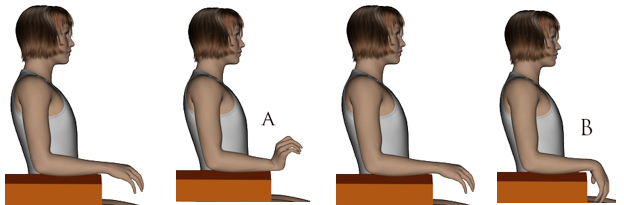
\includegraphics[width=\textwidth,keepaspectratio]{hand-extension-movements.png}
			\centering
			\caption{Exercicis de flexo-extensió de la mà.}
		\end{figure}
		\item[Mobilitat dels dits] amb la mà oberta, separar els dits en forma de ventall tot el possible i mantenir la posició 5-10 segons i tornar a la posició inicial de repòs.
		\begin{figure}[H]
			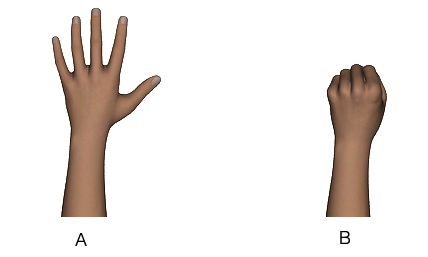
\includegraphics[width=\textwidth,keepaspectratio]{fingers-movility.jpg}
			\centering
			\caption{Exercicis d'extensió dels dits.}
		\end{figure}
		\item[Oposició del polze] dur el palpís del dit polze a la base de cada un dels altres dits començant per l'índex i acabant pel dit petit.
		\begin{figure}[H]
			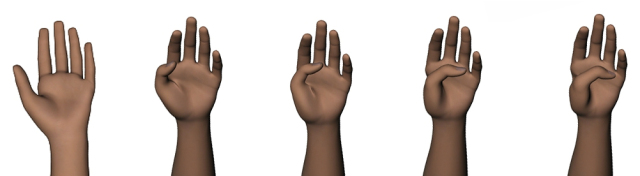
\includegraphics[width=\textwidth,keepaspectratio]{thumb-movility.jpg}
			\centering
			\caption{Exercicis d'oposició del polze.}
		\end{figure}
		\item[Mobilitat lateral del canell] amb la mà oberta, i els dits estirats, realitzar moviments amb el canell dirigint la mà primer cap a fora, mantenir 5-10 segons per a posteriorment relaxar tornant a la posició de repòs. Continuar movent la mà cap a dins, mantenir uns altres 5-10 segons i tornar a la posició inicial.
		\begin{figure}[H]
			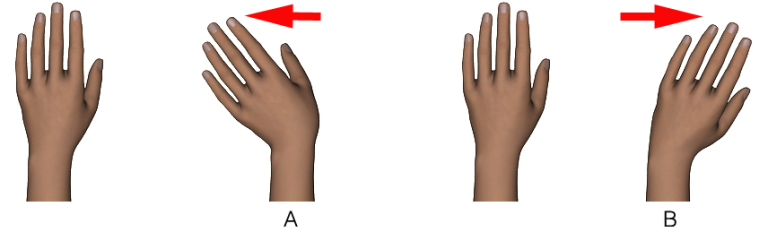
\includegraphics[width=\textwidth,keepaspectratio]{wrist-movility.jpg}
			\centering
			\caption{Exercicis de mobilitat lateral de la mà.}
		\end{figure}
	\end{description}
	\subsection{Interfícies basades en visió per a rehabilitació}
	En aquesta subsecció ens centrarem en el treball relacionat amb VBI que empren directament el moviment del cos sense la necessitat d'emprar comandaments.
	L'ús de \textit{Microsoft Kinect} (o sistemes parescuts com l'\textit{Asus Xtion}) s'han emprat per la rehabilitació de pacients amb accidents vasculars cerebrals, treball d'equilibri o que simplement necessiten recuperació física.
	
	En concret, \textit{Kinect}, presenta un grau d'utilització molt gran en aquests àmbits. \textit{Webster i Celik} \cite{webster-celik}, presenten un recull de treballs que utilitzen \textit{Kinect} per al cuidat de persones majors, per a la rehabilitació de pacients amb accidents vasculars cerebrals i exercicis basats en videojocs. Amb aplicacions tan diverses que van des de la detecció de caigudes en el cas de persones majors, fins aplicacions destinades a ajudar a que els exercicis de rehabilitació repetitius siguin més entretenguts. En el cas dels exercicis basats en videojocs, un dels treballs estudiats presenta un joc per treballar exercicis d'equilibri. En aquest joc, en el que jugador està representat per una figura humana virtual, uns contorns de figures humanes es movien cap al jugador virtual, que havia de imitar els contorns per tal de passar a través d'ells sense tocar-los.
	
	En referència a la rehabilitació de la mà, Leap motion s'empra gràcies a la informació que ens pot donar dels dits i de la posició de la mà. Emprant aquest tecnologia, Liu et al (2015) \cite{liu-rehab} presenten un sistema on el metge pot prescriure al pacient certs moviments per imitar i aquest pot obtenir retroalimentació automàtica en forma de puntuació, d'acord amb la similitud. També es troba la utilització de videojocs per complementar la teràpia convencional (Iosa et al., 2015) \cite{losa-rehab}. Matos et al (2014) \cite{kinteract} presenten un joc per entrenar el rang d'obertura de la mà, l'usuari ha d'obrir la mà per recollir pomes i transportar-les a una cistella mantenint l'obertura de la mà. Khademi et al. (2014) juguen al Fruit Ninja emprant  la mà a rehabilitar per pacients amb accidents vascular cerebrals \cite{leap-fruit-ninja}.
	\section{Anàlisi i disseny}
	\subsection{Introducció}
	Dins aquest apartat s'analitza i descriu quin ha estat el sistema desenvolupat per tal de satisfer els objectius plantejats anteriorment.
	
	En primer lloc es presenta una descripció de l'arquitectura i les característiques del controlador Leap Motion, que serà la interfície basada en visió que s'emprarà.
	
	Posteriorment es fa una anàlisi de requisits del sistema a desenvolupar tant des del punt de vista funcional com tecnològic, la qual cosa permet tenir una descripció detallada del sistema.
	
	Com a darrera secció es descriu el disseny de l'aplicació amb tots els seus subsistemes i els diferents jocs desenvolupats.
	\subsection{Leap Motion}
	\subsubsection{Hardware: Leap motion}
	El \textit{Leap motion} és un petit dispositiu que es connecta mitjançant USB i que és capaç de capturar els moviments de mans i dits, així com gestos o moviments de llapis (stylus) a través de dues càmeres i tres LEDs infraroigs. El dispositiu és capaç de capturar les dades de les mans fins a una distància d'uns 60 cm, tant a la part superior com als laterals del dispositiu, gràcies al gran camp de visió de les càmeres (uns 150\textdegree) \cite{leapcharacteristics}.
	\begin{figure}[H]
		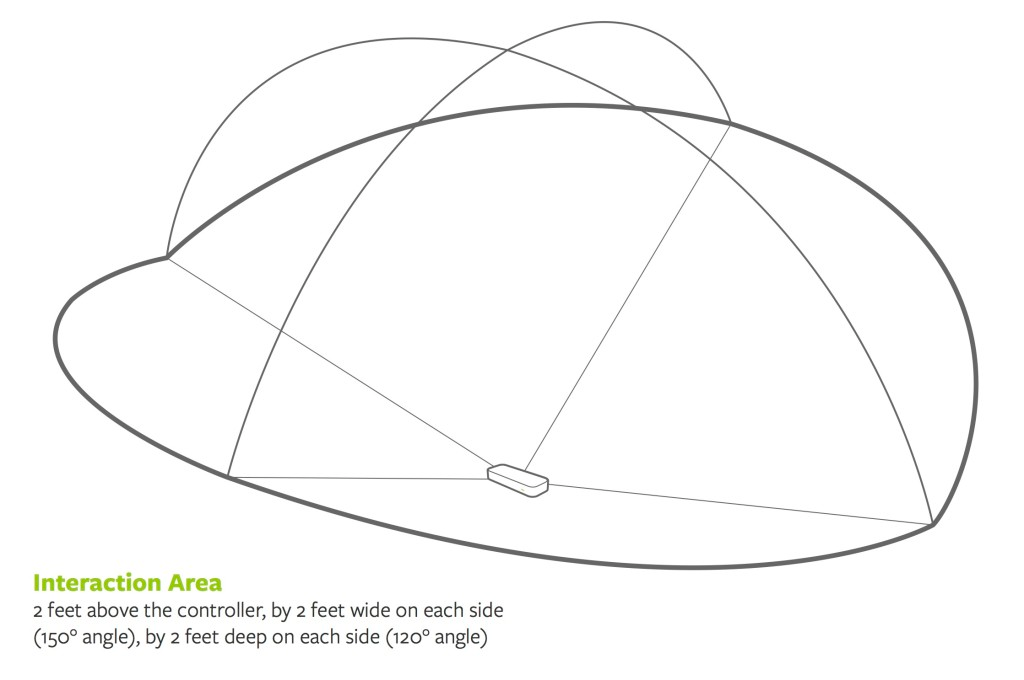
\includegraphics[width=\textwidth,keepaspectratio]{leap-motion-interaction-area.png}
		\centering
		\caption{Representació del dispositiu i el seu camp de visió \protect\cite{leapcharacteristics}.}
	\end{figure}
	Les dades capturades per aquestes càmeres són enviades per USB a l'ordinador al qual es connecta el controlador Leap, on el software de Leap Motion, que s'executa com un servei, s'encarrega de processar-les i deixar-les disponibles perquè puguin ser obtingudes mitjançant APIs.
	
	El servei del \textit{Leap Motion} proporciona la informació a les APIs en forma d'una sèrie de fotogrames que contenen tota la informació de seguiment capturada. Al final és competència d'aquestes APIs proporcionar a l'usuari les dades en forma d'estructures orientades a objectes, així com també proporcionar una sèrie de funcions que permeten operar amb aquestes dades.
	\subsubsection{Arquitectura del Leap Motion}
	El \textit{Leap Motion} és capaç de funcionar en múltiples sistemes operatius i les seves dades poden ser obtingudes de dues formes: mitjançant una interfície nativa o a través d'un servidor de \textit{Web socket}. D'aquesta manera, les possibilitats per als desenvolupadors són molt diverses i inclouen molts dels llenguatges de programació més utilitzats actualment \cite{leapsdkdocs}.
	
	\paragraph{Interfície nativa}
	La interfície nativa es proporciona a través d'una llibreria que connecta el servei del \textit{Leap Motion}. Aquest servei després proveeix les dades de seguiment obtingudes a les aplicacions desenvolupades. La llibreria es pot utilitzar directament en el cas d'aplicacions desenvolupades amb C++ i Objective C, o es poden utilitzar una de les APIs per Java, C\# o \textit{Python} \cite{leapsdkdocs}.
	\begin{figure}[H]
		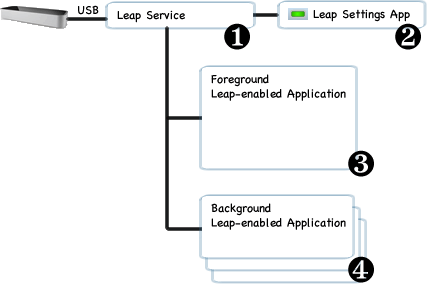
\includegraphics[width=\textwidth,keepaspectratio]{native-interface.png}
		\centering
		\caption{Esquema d'aplicacions utilitzant la interfície nativa.}
		\label{fig:native-interface}
	\end{figure}
	A continuació es descriuen les diferents parts que intervenen en la connexió del dispositiu mitjançant la interfície nativa representada a la figura \ref{fig:native-interface}.
	\begin{enumerate}
		\item El servei de \textit{Leap Motion} rep les dades del controlador a través d'una connexió USB, processa les dades rebudes i les envia a les aplicacions. Per defecte el servei només envia informació a les aplicacions en primer pla, però les aplicacions poden demanar rebre dades també en segon pla.
		\item L'aplicació de \textit{Leap Motion} és independent del servei i permet als usuaris configurar la seva instal·lació de \textit{Leap Motion}.
		\item Una aplicació en primer pla rep dades de seguiment del servei de \textit{Leap Motion}.
		\item Quan una aplicació perd el focus del sistema operatiu, el servei de \textit{Leap Motion} deixa d'enviar-li dades. Les aplicacions dissenyades per funcionar en segon pla poden demanar al servei que els proveeixi dades de seguiment fins i tot en segon pla.
	\end{enumerate}
	
	\paragraph{Interfície web socket}
	El servei de Leap Motion executa un servidor de \textit{web socket} local en el domini local (\textit{localhost}) a través del port 6437. Aquesta interfície de web socket proveeix dades de seguiment en format JSON. Després un client \textit{JavaScript} desenvolupat per la mateixa empresa de Leap Motion, s'encarrega de capturar aquestes dades i presentar-les com a objectes de \textit{JavaScript} estàndard.
	\begin{figure}[H]
		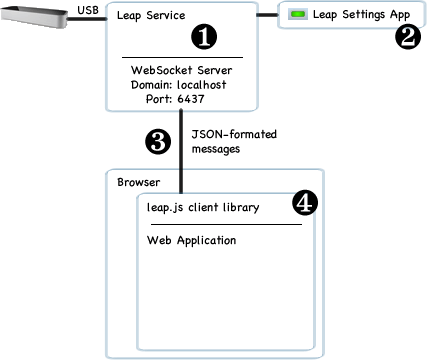
\includegraphics[width=\textwidth,keepaspectratio]{websocket-interface.png}
		\centering
		\caption{Esquema d'aplicacions utilitzant la interfície de web socket.}
		\label{fig:websocket-interface}
	\end{figure}
	Tot seguit es descriuen les diferents parts que intervenen en la connexió del dispositiu mitjançant \textit{web socket}, representat a la figura \ref{fig:websocket-interface}
	\begin{enumerate}
		\item El servei de \textit{Leap Motion} proveeix un servidor de \textit{web socket} a través de la direcció \textit{http://127.0.0.1:6437}.
		\item L'aplicació de configuració del \textit{Leap Motion} permet habilitar o deshabilitar el servidor de \textit{web socket}.
		\item El servidor envia les dades de seguiment en format JSON. Les aplicacions també poden enviar missatges de configuració al servidor.
		\item La mateixa empresa de \textit{Leap Motion} ens proveeix d'una llibreria \textit{JavaScript} que pot ser utilitzada per les aplicacions web per accedir a les dades de seguiment del \textit{Leap Motion}.
	\end{enumerate}
	Aquesta interfície està dissenyada per ser utilitzada per aplicacions web, tot i que qualsevol aplicació pot establir una connexió amb el servidor de web socket. Aquest servidor segueix l'estàndard de web socket RFC6455.
	\subsubsection{Leap Motion API}
	El sistema \textit{Leap Motion} realitza un seguiment de les mans i els dits. El dispositiu ofereix una gran precisió i una alta taxa de fotogrames per segon, i retorna valors discrets de posició i moviment.
	
	Els sensors es dirigeixen cap a l'eix Y, (cap amunt, quan el controlador es situa en la seva posició de funcionament estàndard) i com s'ha comentat anteriorment, ofereix un camp de visió d'uns 150\textdegree.
	\paragraph{Sistema de coordenades}
	El sistema \textit{Leap Motion} utilitza un sistema de coordenades cartesianes. L'origen d'aquest sistema de coordenades es situa a la part superior del dispositiu. Els eixos X i Z es situen en el pla horitzontal, amb l'eix X paral·lel a l'eix més llarg del dispositiu. L'eix Y és vertical amb valors més positius cap amunt. L'eix Z té valors positius en direcció a l'usuari i valors negatius del dispositiu en direcció contraria a l'usuari.
	\begin{figure}[H]
		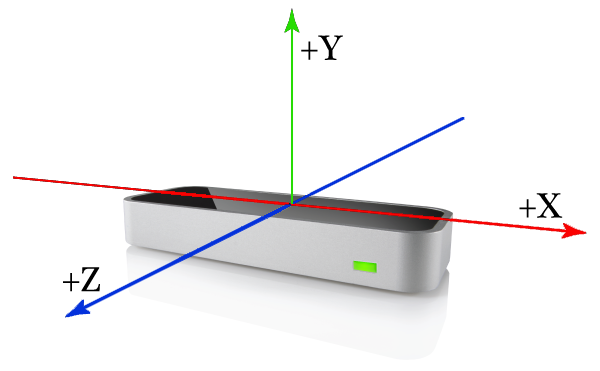
\includegraphics[width=\textwidth,keepaspectratio]{leap-coordinates.png}
		\centering
		\caption{Sistema de coordenades del Leap Motion.}
		\label{fig:leap-coordinates}
	\end{figure}
	La API mesura les quantitats físiques en les següents unitats.\\
	
	\begin{tabular}{ l c l }
		\hline
		Distància & & milimetres\\ \hline
		Temps & & microsegons\\ \hline
		Velocitat & &  milimetres / segon\\ \hline
		Angles & & Radians\\
	\end{tabular}
	
	\vspace{5mm}
	Mentre el dispositiu fa un seguiment de les mans i dits en el seu camp de visió, proveeix actualitzacions de les dades com un conjunt de fotogrames (\textit{frames}) de dades. cada objecte \textit{frame} conté qualsevol mà detectada, detallant les seves propietats en un únic instant de temps. L'objecte \textit{Frame} és esencialment, l'origen del model de dades retornat per la API.
	Aquesta posa a disposició dels desenvolupadors les següents classes.
	
	\paragraph{Hands}
	Les mans es representen mitjançant la classe \textit{Hand} i proveeix informació sobre la identitat, posició i altres característiques de la mà detectada. Llista també tots els dits, així com també el braç al qual està lligada la mà.
	\begin{figure}[H]
		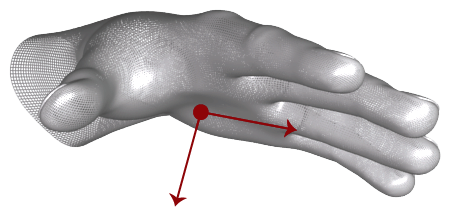
\includegraphics[width=\textwidth,keepaspectratio]{leap-hand-model.png}
		\centering
		\caption{Representació d'una mà i els vectors palmNormal i direction.}
		\label{fig:leap-hand}
	\end{figure}
	El software del \textit{Leap Motion} utilitza un model intern de la mà per tal d'oferir un seguiment predictiu, fins i tot quan parts de la mà no són visibles per els sensors. La classe \textit{Hand} ofereix una propietat \textit{Hand.confidence}, que indica en quin nivell d'exactitud encaixa en el model intern, la mà detectada.
	
	Tot i que el dispositiu és capaç de detectar més de dues mans si més d'una persona està dins el camp de visió. Es recomana limitar les mans a dues per maximitzar la qualitat de les dades de seguiment.
	\paragraph{Arms}
	\textit{Hand.arm} és un objecte que proporciona informació sobre l'orientació, longitud, amplada i punts finals d'un braç. Quan el colze està fora del camp de visió el sistema estima la posició del braç basant-se en observacions passades, així com amb les proporcions normals d'un braç humà.
	\paragraph{Fingers}
	Proporciona informació de cada dit de la mà. En cas que part d'un dit, o fins i tot tot el dit, no sigui visible, les característiques s'estimen en base a observacions recents i del model intern de la mà. Aquests dits s'identifiquen amb el seu nom en anglès (\textit{thumb}, \textit{index}, \textit{middle}, \textit{ring} i \textit{pinky}).
	\begin{figure}[H]
		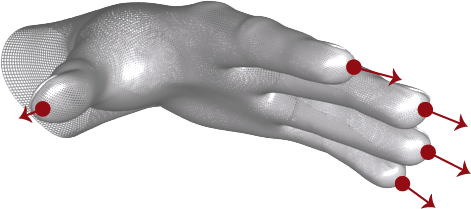
\includegraphics[width=\textwidth,keepaspectratio]{leap-fingers-model.png}
		\centering
		\caption{Representació d'una mà i els vectors de direcció dels dits.}
		\label{fig:leap-hand-fingers}
	\end{figure}
	Els objectes del tipus \textit{Finger} conté objectes de la classe \textit{Bone} que descriuen la posició i orientació de cada os del dit. Tots els dits contenen 4 ossos, ordenats de la base a la punta dels dits.
	\begin{figure}[H]
		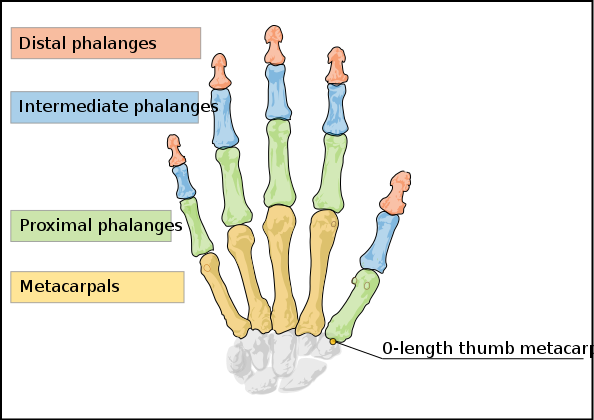
\includegraphics[width=\textwidth,keepaspectratio]{hand-bones.png}
		\centering
		\caption{Representació dels diferents ossos de la classe Hand.}
		\label{fig:hand-bones}
	\end{figure}
	Els ossos s'identifiquen de la següent manera:
	\begin{description}
		\item[Metacarpal] el \textit{metacarpal} (metacarpià) és l'os situat dins la mà, que connecta el dit al canell (excepte el polze).
		\item[Proximal Phalanx] \textit{proximal phalanx} (primera falange) és l'os de la base del dit, connectat al palmell.
		\item[Intermediate Phalanx] l'\textit{intermediate phalanx} (segona falange) és l'os intermig del dit, situat entre la punta i la base del dit.
		\item[Distal Phalanx] el \textit{distal phalanx} (tercera falange) és el darrer os del dit, situat a la punta del dit.
	\end{description}
	Per mantenir una coherència, el model del polze no reflecteix el model anatòmic real. Un polze real té un os menys que la resta de dits, en canvi el model retornat per la API conté un metacarpià de longitud 0 per tal de tenir el mateix numero d'ossos que la resta de dits.
	\subsection{Requeriments}
	Tot i que l'objectiu principal del projecte és realitzar una prova de concepte per confirmar que és possible utilitzar el controlador \textit{Leap Motion} per complementar i monitorar teràpies de rehabilitació, és important establir una sèrie de requeriments tècnics i funcionals del projecte per tal de definir bé el seu abast.
	\subsubsection*{Requeriments d'usuari}
	\begin{description}
		\item [RU1] Un usuari ha de poder seleccionar un exercici a realitzar d'una llista.
		\item [RU2] Un usuari ha de poder realitzar exercicis d'extensió del canell.
		\item [RU3] Un usuari ha de poder realitzar exercicis d'abducció i adducció del canell.
		\item [RU4] Un usuari ha de poder realitzar exercicis d'abducció i adducció dels dits.
		\item [RU5] Un Responsable de la rehabilitació d'un usuari ha de ser capaç de reproduir les sessions d'exercicis dels usuaris.
	\end{description}
	\subsubsection*{Requeriments funcionals dels jocs}
	\begin{description}
		\item [RF1] Els jocs han de ser el més intuïtius possibles.
		\item [RF2] Els jocs han d'engrescar als usuaris a realitzar els exercicis.
		\item [RF3] Els jocs han d'enviar les dades de seguiment dels moviments.
		\item [RF4] Cada joc ha de permetre als usuaris realitzar un sol exercici.
	\end{description}
	\subsubsection*{Requeriments no funcionals}
	\begin{description}
		\item [RNF1] Els jocs han de poder ser executats a qualsevol sistema operatiu.
		\item [RNF2] Els usuaris no han d'instal·lar cap aplicació addicional llevat dels controladors del dispositiu \textit{Leap Motion}.
	\end{description}
	\subsection{Arquitectura del sistema}
	Una vegada definits els requeriments del projecte, a continuació es presenta una descripció de l'arquitectura dissenyada per tal de satisfer aquests requeriments.
	
	Un dels objectius ha estat des del primer moment que l'accés a l'aplicació fos el més fàcil possible per part dels usuaris. Per això es va decidir que el millor era que les aplicacions s'executassin en un entorn web.
	
	Una aplicació web te l'avantatge de ser multiplataforma, és independent del sistema operatiu que tingui l'usuari el qual facilita l'accés a l'aplicació.
	
	En el nostre cas s'utilitza una una arquitectura web tradicional que consta d'un servidor web que és l'encarregat de servir les aplicacions de rehabilitació als usuaris. Aquestes aplicacions contenen la major part de la lògica de l'aplicació. L'arquitectura presenta una peculiaritat, fora del que és una aplicació web tradicional, que és la utilització d'un servidor de \textit{web socket} que és l'encarregat de rebre les dades del dispositiu \textit{Leap Motion} dels usuaris i guardar aquestes dades en fitxers per a que puguin ser reproduïts posteriorment pels responsables de les teràpies de rehabilitació.\\
	
	// grafic de l'arquitectura de l'aplicació
	
	\begin{description}
		\item [Aplicacions web de rehabilitació] aquestes aplicacions són les encarregades de connectar-se al dispositiu \textit{Leap Motion} dels usuaris per tal que aquests puguin realitzar els exercicis.
		\item [Servidor web] un servidor web tradicional encarregat de servir les pagines web als usuaris. També ha de ser l'encarregat de gestionar totes les dades dels usuaris per a que els responsables de la teràpia puguin fer un seguiment de les sessions de rehabilitació dels usuaris.
		\item [Servidor web socket] és un servidor que habilita una comunicació bidireccional en temps real amb els usuaris. Aquest servidor s'encarrega de guardar les dades enviades pels dispositius \textit{Leap Motion} dels usuaris per tal que aquestes puguin ser monitorades posteriorment.
	\end{description}
	\subsection{Disseny dels jocs}
	Per tal de satisfer els requeriments plantejats anteriorment, s'han dissenyat tres jocs diferents.
	
	Cada joc està dissenyat per treballar un tipus d'exercici determinat. Això implica que la complexitat del joc no pot ser molt elevada, ja que el control que pot arribar a tenir l'usuari sobre el joc, realitzant una mateixa acció repetidament és baix. A més, no s'ha d'oblidar que l'objectiu principal dels jocs no és el simple entreteniment de l'usuari, sinó que el més important és que l'usuari es senti motivat per realitzar els exercicis de rehabilitació i els realitzi de manera correcta.
	
	A més s'ha desenvolupat una aplicació de monitoratge, que podria ser utilitzada pels responsables de de la rehabilitació per dur a terme un seguiment de l'evolució dels usuaris.
	\subsubsection{Runner boy - Exercici d'extensió del canell}
	Aquest joc està específicament dissenyat per treballar el moviment d'extensió del canell.
	És un joc de desplaçament lateral infinit on l'usuari agafa el control d'una persona o jugador, que va corrent per l'escenari del joc com es mostra a la figura \ref{fig:runnerboy-simple}.
	\begin{figure}[H]
		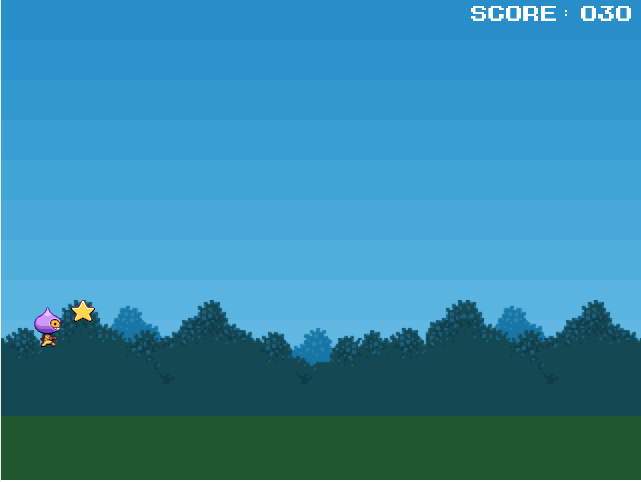
\includegraphics[width=0.8\textwidth,keepaspectratio]{runner-boy-simple.png}
		\centering
		\caption{Imatge del jugador saltant per capturar una estrella.}
		\label{fig:runnerboy-simple}
	\end{figure}
	L'objectiu és capturar unes estrelles que van apareixent en direcció contraria a l'usuari per obtenir punts. Per tal d'afegir complexitat al joc també apareixen uns obstacles que l'usuari ha d'esquivar per no perdre la partida. A més a mesura que la puntuació de l'usuari es va incrementant, també ho fa la velocitat a la que es desplaça el joc, tant els obstacles com les estrelles de puntuació.
	L'usuari controla el joc per mitjà del dispositiu Leap Motion. El primer té la capacitat de fer botar el jugador, per tal d'obtenir les estrelles que s'acosten per l'aire o d'esquivar els obstacles que apareixen per terra, tal com es mostra a la figura \ref{fig:runnerboy-obstacle}.
	\begin{figure}[H]
		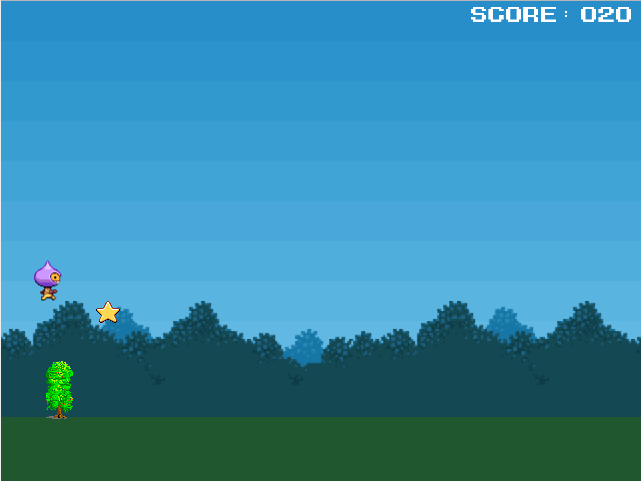
\includegraphics[width=0.8\textwidth,keepaspectratio]{runner-boy-obstacle.png}
		\centering
		\caption{Imatge del jugador esquivant un obstacle durant la partida.}
		\label{fig:runnerboy-obstacle}
	\end{figure}
	El jugador realitza el moviment de salt quan l'usuari estén el canell, elevant els dits de la mà per sobre del canell tant com li sigui possible.
	\subsubsection{Cubes road - Exercici d'abducció i adducció del canell}
	En aquest joc, els usuaris treballen els moviments d'abducció i adducció del canell de la mà. Es tracte d'un joc en 3 dimensions, en el que uns cubs es mouen a través d'una carretera en direcció a l'usuari, aquest ha d'intentar capturar-los desplaçant lateralment un altre cub.
	
	L'objectiu del joc és capturar la major quantitat de cubs possibles, incrementant així la puntuació de l'usuari. A mesura que la puntuació de l'usuari augmenta, també ho fa la velocitat a la que es desplacen els objectes cap a ell augmentant així la dificultat del joc.
	\begin{figure}[H]
		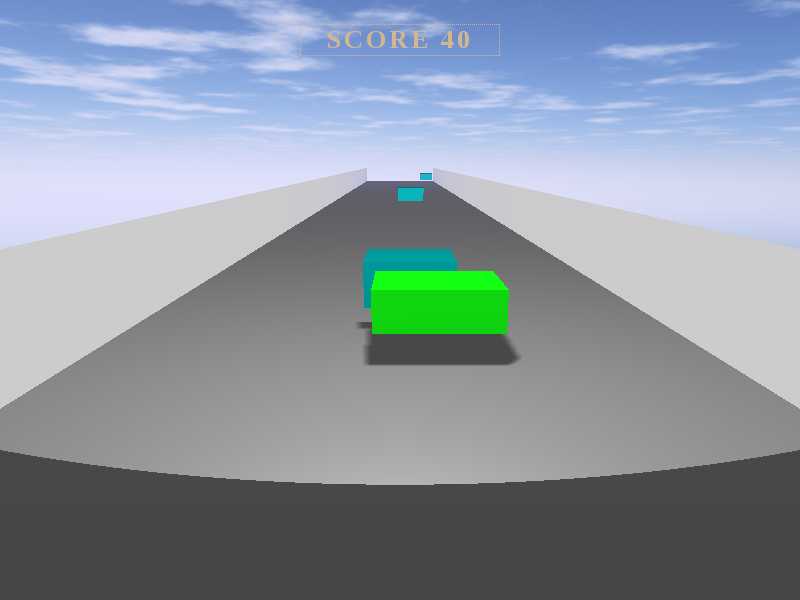
\includegraphics[width=0.8\textwidth,keepaspectratio]{cubes-road-simple.png}
		\centering
		\caption{Situació normal del joc.}
		\label{fig:cubes-road-simple}
	\end{figure}
	Amb l'objectiu d'augmentar la complexitat del joc i la motivació dels usuaris, periòdicament van apareixent uns cubs d'un color diferent que l'usuari haurà d'esquivar. En cas que l'usuari sigui incapaç d'esquivar algun d'aquests cubs que podríem denominar cubs enemics, la mida del cub que utilitza l'usuari per capturar els objectes es va reduint, d'aquesta manera com més errors comet l'usuari més difícil és per ell seguir amb la partida.
	
	La figura següent mostra l'estat del jugador després d'haver capturat per error varis cubs enemics, així com l'aspecte d'un d'aquests cubs enemics.
	\begin{figure}[H]
		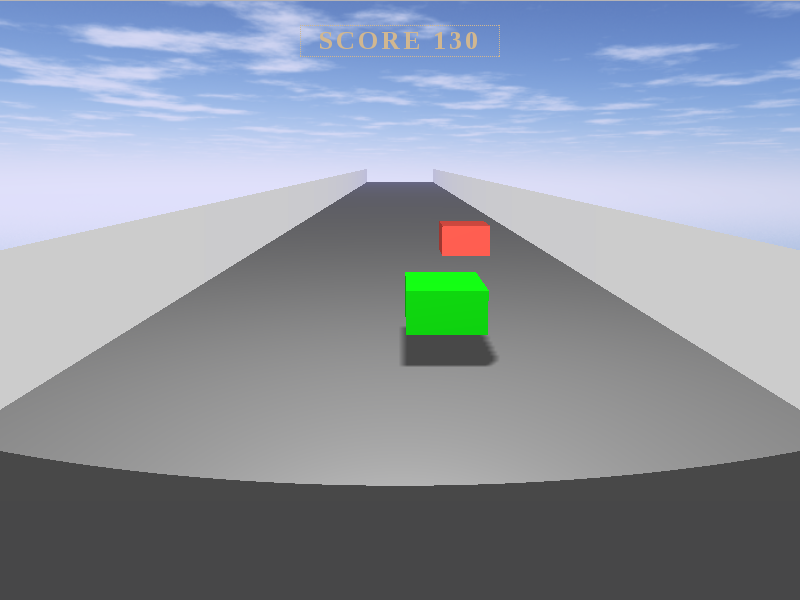
\includegraphics[width=0.8\textwidth,keepaspectratio]{cubes-road-enemy.png}
		\centering
		\caption{Imatge del jugador després d'haver col·lisionat amb varis enemics.}
		\label{fig:cubes-road-enemy}
	\end{figure}
	El moviment horitzontal del cub capturador (verd) es duu a terme mitjançant moviments d'abducció i adducció de la mà.
	\subsubsection{Catch stars - Exercici d'abducció i adducció del dits}
	\subsection{Leap networking plugin}
	\subsection{Aplicació de monitorització}
	Aquesta aplicació permet als responsables de les teràpies de rehabilitació monitoritzar les sessions d'exercicis que fan els seus pacients. D'aquesta manera un responsable pot avaluar la millora d'un pacient. De la mateixa manera es poden detectar errors en la realització dels exercicis.
	
	L'aplicació de monitorització consta de 3 parts fonamentals, un plugin del controlador Leap Motion, un servidor de web socket i una aplicació de reproducció dels moviments capturats pel controlador Leap del pacient. La següent figura mostra un esquema de l'arquitectura de l'aplicació de monitorització.
	\begin{figure}[H]
		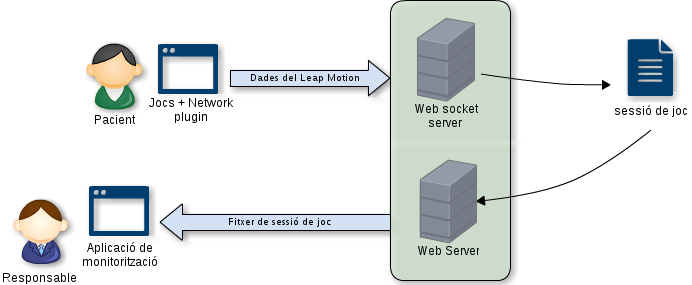
\includegraphics[width=0.8\textwidth,keepaspectratio]{esquema-monitoritzacio.png}
		\centering
		\caption{Arquitectura de l'aplicació de monitorització.}
		\label{fig:arquitectura-monitoritzacio}
	\end{figure}
	Així, un pacient es connecta a un dels jocs definits anteriorment, mentre l'usuari juga, un plugin del Leap Motion va enviantles dades capturades a un servidor de web socket utilitzant una estructura determinada, a la vegada, aquest servidor s'encarrega de guardar les dades rebudes a un fitxer. Després en un altre moment, un dels responsables de la teràpia d'aquest pacient, es connecta a l'aplicació de monitorització per tal de reproduir la sessió de joc del seu pacient. En aquest cas el servidor web l'unic que fa es servir les aplicacions als usuaris i el fitxer de la sessió de joc cap a l'aplicació de monitorització.
	\begin{description}
		\item[Network plugin] aquest és un plugin que segueix la mateixa filosofia que els plugins ja disponibles pel Leap Motion \cite{leapjsplugins}. El primer que fa el plugin és connectar-se a un servidor de web socket. Després quan el controlador Leap Motion comença a enviar dades, aquest plugin les captura i les envia al servidor de socket utilitzant una estructura determinada.
		\item[Web socket] un servidor de web socket tradicional que accepta connexions del plugin del Leap Motion i escolta els esdeveniments d'aquestes connexions. Quan rep una connexió nova, crea un fitxer de text i una vegada creat el fitxer de text, va escrivint les dades rebudes a través del socket al fitxer de text en format JSON. Una vegada que el plugin tanca la connexió amb el servidor, aquest darrer reb un esdeveniment de desconnexió i deixa el fitxer disponible per a ser reproduït per l'aplicació de monitorització.
		\item[GUI de monitorització] és una aplicació web que es connecta al controlador Leap Motion, i utilitza les dades del fitxer, creat per el servidor de socket, per reproduir els moviments de la mà que ha realitzat l'usuari del joc.
		
		Com si es tractàs d'un fitxer de video, aquesta aplicació permet pausar la reproducció dels moviments, així com moure's endavant i enrere. Per tal de facilitar la revisió dels moviments, els usuaris d'aquesta aplicació també tenen la capacitat de rotar la mà que es veu a la reproducció i modificar el zoom de la imatge.
	\end{description}
	\section{Implementació}
	En aquest apartat es descriuen els detalls d'implementació de les diferents aplicacions i sistemes desenvolupats.
	Primer, es presenten les tecnologies utilitzades per desenvolupar les aplicacions i les raons per les quals s'han triat aquestes tecnologies, i després es detallen els aspectes més interessants de la implementació de les diferents aplicacions.
	
	\subsection{Tecnologies utilitzades}
	Durant l'implementació de les aplicacions i sistemes dissenyats s'han utilitzat les següents tecnologies i llenguatges de programació.
	\begin{description}
		\item[HTML, CSS] són la base de l'estructura i el disseny de qualsevol aplicació web.
		\item[JavaScript] és el llenguatge de programació utilitzat pels navegadors web.
		\item[Node.js] és un entorn multiplataforma que permet executar codi JavaScript a la banda del servidor. Presenta una arquitectura basada en esdeveniments i que permet l'execució d'operacions d'entrada i sortida de manera asíncrona. Aquestes prestacions tenen l'objectiu de maximitzar la productivitat d'aplicacions amb múltiples operacions d'entrada i sortida, així com facilitar l'implementació d'aplicacions web de temps real \cite{nodejs}.\\
		Aquestes característiques fan que aquesta tecnologia sigui una de les més adecuades per a la implementació del servidor de web socket, ja que aquesta rebrà moltes peticions i haurà de realitzar operacions d'escritura per a cada petició.
	\end{description}
	Per altra banda s'han utilitzat diverses llibreries que han ajudat a implementar les diferents aplicacions, en especial a l'hora la programació dels videojocs.\\
	\begin{description}
		\item[Express.js] és un framework per al desenvolupament de servidors web amb Node.js.
		\item[Socket.io] és una llibreria per a JavaScript per a l'implementació d'aplicacions web de temps real. Consta de dues parts, una llibreria client que s'executa al navegador i una llibreria per al servidor (Node.js). Proporciona un gran ventall de prestacions al voltant de web socket.
		\item[Phaser.io] és una llibreria per al desenvolupament de videojocs HTML5 en 2d.
		\item[Three.js] és una llibreria JavaScript que permet la creació de gràfics en 3 dimensions per a navegadors web.
		\item[Physijs] és un plugin per a Three.js que facilita la gestió de càlculs físics. Afegeix prestacions com gravetat, gestio de colisions, rebots, etc, a una escena de three.js.
		\item[TweenMax] és una llibreria per a la gestió d'animacions complexes en Javascript.
		\item[Leapjs Plugin] Plugin per al software de Leap Motion per a JavaScript que permet la reproducció dels fotogrames capturats per el controlador Leap Motion. Utilitzat en l'implementació de l'aplicació de monitorització.
	\end{description}
	\subsection{Detalls d'implementació}
	Per al desenvolupament del projecte i la consecució dels objectius prevists, s'han implementat els següents sistemes i aplicacions.
	\begin{description}
		\item[Servidor web] encarregat de servir les aplicacions web i els fitxers estàtics necessaris per el funcionament d'aquestes.
		\item[Servidor web socket] Utilitzat per guardar les dades de seguiment dels dispositius Leap Motion dels usuaris, per tal que puguin ser reproduïts posteriorment quan es desitgi.
		\item[Runner boy] videojoc HTML5 desenvolupat utilitzant la llibreria Phaser.io. Està dedicat a exercitar el moviment de flexió del canell.
		\item[Cubes Road] videojoc HTML5 en 3D desenvolupat utilitzant la llibreria Three.js. Té com a objectiu exercitar els moviments d'abducció i adducció del canell.
		\item[Catch Stars] videojoc HTML5 desenvolupat únicament amb l'element HTML5 canvas. L'objectiu principal d'aquest joc és exercitar els moviments d'abducció i adducció dels dits cor i anular. D'altra banda un altre objectiu d'implementar el joc utilitzant només la API dels elements canvas, ha estat comparar com és la creació d'un videojoc utilizant APIs bàsiques com les de canvas, en vers a l'utilització de llibreries com Phaser.io i Three.js que faciliten molts processos.
		\item[LeapJS Network plugin] Plugin propi desenvolupat seguint la filosofia dels plugins ja disponibles per Leapjs. La seva funció és enviar les dades de seguiment del controlador Leap Motion, a un servidor de web socket.
		\item[Aplicació de monitorització] Una aplicació web que utilitza el plugin leapjs-playback per reproduir les dades de seguiment del Leap Motion. Per tal de reproduir els moviments, utilitza el fitxer guardat pel servidor de web socket.
	\end{description}
	A continuació es descriuen de manera detallada els aspectes més interessants de la implementació d'aquests sistemes i aplicacions.
	\subsubsection{Servidoer web}
	\subsubsection{Servidor socket}
	Aquest servidor, desenvolupat mitjançant la llibreria Socket.io, s'encarrega de rebre les connexions del plugin de Leap Motion i generar els fitxers de les sessions de joc.\\
	El seu paper més important és generar el fitxer de les sessions de joc utilitzant l'estructura adecuada, que després podrà ser reproduida utilitzant el plugin de reproducció “leapjs-playback”. A continuació es mostra quina és l'estructura de dades que ha de guardar el servidor de web socket en el fitxer.
	\begin{figure}[H]
	\begin{lstlisting}[]
	{
	  metadata: {
	    formatVersion: 2,
	    generatedBy: 'Socket.io saver',
	    frames: 0,
	    protocolVersion: 6,
	    frameRate: '1.1e+2',
	    modified: new Date()
	  },
	  frames: [packingStructure]
	}
	\end{lstlisting}
		\caption{Estructura del fitxer de sessió de joc.}
		\label{fig:recording-structure}
	\end{figure}
	Les meta dades venen determinades pel plugin de reproducció y la majoria són constants o són regenerades a l'hora de reproducció del plugin, com és el cas del “frameRate” (ratio de fotogrames).
	
	Les dades de seguiment del Leap es guarden en forma de “Array” de fotogrames a la propietat “frames”, amb l'unica peculiaritat que el primer element de la “Array” descriu l'estructura amb que es guarda cada fotograma. Aquest estructura amb que es guarda cada fotograma serà descrita a l'apartat de “Network Plugin”, ja que és el plugin desenvolupat el que s'encarrega de generar les dades amb l'estructura adequada i enviar-les.
	
	El Servidor utilitza el que Socket.io defineix com a “namespace” per tal d'atendre les connexions de cada un dels jocs. Un “namespace” es pot entendre com una sala en la que els sockets es poden comunicar entre si, d'aquesta manera un servidor pot enviar missatges a tots els sockets connectats a una sola sala i només als d'aquella sala.
	Es defineix una sala per a cada videojoc, d'aquesta menera:
	\begin{figure}[H]
	\begin{lstlisting}[]
	io.of('/catch-stars')
	  .on('connection', leapRecorder);
	io.of('/runner-boy')
	  .on('connection', leapRecorder);
	io.of('cubes-road')
	  .on('connection', leapRecorder);
	\end{lstlisting}
		\caption{Sales del servidor de socket}
		\label{fig:socket-namespaces}
	\end{figure}
	Com es pot veure totes les connexions a les diferents sales, són manegades per la mateixa funció “leaprecorder”. Tot i que pot parèixer innecessari crear una sala per a cada videojoc, d'aquesta manera és més fàcil generar fitxers amb noms diferents per a cada videojoc, a més el codi queda més estructurat de cara al futur.
	La funció “leapRecorder” reb com a parametre un objecte Socket i serà a través d'aquest que es rebran els esdeveniments enviats pel plugin.
	\begin{figure}[H]
	\begin{lstlisting}[]
	function leapRecorder(socket){
	  let fileName = socket.id.substring(socket.nsp.name.length + 1);
	  fileName = socket.nsp.name.substring(1) + '-' + fileName + '.json';
	  const ws = fs.createWriteStream(fileName);
	  const fileData = {
	    metadata: {
	      formatVersion: 2,
	      generatedBy: 'Socket.io saver',
	      frames: 0,
	      protocolVersion: 6,
	      frameRate: '1.1e+2',
	      modified: new Date()
	    },
	    frames: [packingStructure]
	  }
	  const str = JSON.stringify(fileData);
	  ws.write(str.substring(0, str.length - 2));
	
	  socket.on('disconnect', () => {
	    ws.write(']}');
	    ws.close();
	  });
	
	  socket.on('frameBuffer', data => {
	    let buffer = JSON.stringify(data[0]);
	    for (let i = 1; i < data.length; i++) {
	      buffer = buffer + ',' + JSON.stringify(data[i]);
	    }
	    ws.write(',' + buffer);
	  });
	}
	\end{lstlisting}
		\caption{Funció principal del servidor de socket}
		\label{fig:socket-namespaces}
	\end{figure}
	Val la pena descriure breument el funcionament d'aquesta funció.
	Quan un client es connecta a al servidor, es crea un fitxer amb l'estructura descrita anteriorment. El fitxer es guarda en format JSON (JavaScript Object Notation, en anglès). En concret, del text resultant de convertir l'objecta a JSON, es guarda tot llevat dels dos darrers caracters.
	\begin{lstlisting}
	ws.write(str.substring(0, str.length - 2));
	\end{lstlisting}
	Això serà el que permetrà anar afegint les dades rebudes periòdicament dins de l'array “frames”, sense haver de regenerar cada vegada l'objecte complet.
	Així, quan el plugin envia un missatge de dades del Leap Motion, aquestes són afegides directament al final del fitxer en format JSON.
	\begin{figure}[H]
	\begin{lstlisting}[]
	socket.on('frameBuffer', data => {
	  let buffer = JSON.stringify(data[0]);
	  for (let i = 1; i < data.length; i++) {
	    buffer = buffer + ',' + JSON.stringify(data[i]);
	  }
	  ws.write(',' + buffer);
	});
	\end{lstlisting}
		\caption{funció que atén les dades de seguiment}
		\label{fig:socket-frame-data}
	\end{figure}
	Com es pot veure, dins missatge de dades del plugin, no arriba només un fotograma capturat per el Leap Motion, sinó que arriben multiples fotogrames. Això s'ha fet així per tal d'optimitzar l'utilització de xarxa del plugin ja que el ratio de fotogrames per segón produït pel controlador Leap Motion, pot ser molt gran.
	
	Finalment, una vegada l'usuari tanca el joc, el servidor detecta la desconnexió de l'usuari i tanca el fitxer. Per tal que el fitxer contingui un JSON ben format, s'han d'afegir els dos caracters que s'han omès a l'inici de la connexió.
	\begin{figure}[H]
	\begin{lstlisting}[]
	socket.on('disconnect', () => {
	  ws.write(']}');
	  ws.close();
	});
	\end{lstlisting}
		\caption{Event de desconnexió}
		\label{fig:socket-disconnect}
	\end{figure}
	Una vegada tancat el fitxer, aquest ja està disponible per a ser reproduït per l'aplicació de monitorització.
	\subsubsection{Runner Boy}
	\subsubsection{Cubes Road}
	\subsubsection{Catch Stars}
	\subsubsection{Network plugin}
	\subsubsection{Aplicació de monitorització}
	\section{Futur}
	\section{Conclusions}
	\printbibliography[heading=bibnumbered,title={Referències}]
\end{document}